\begin{center}
\begin{Huge}Analysis II\end{Huge}\\
\end{center}

\vspace{-2em}
\section{Allgemein}

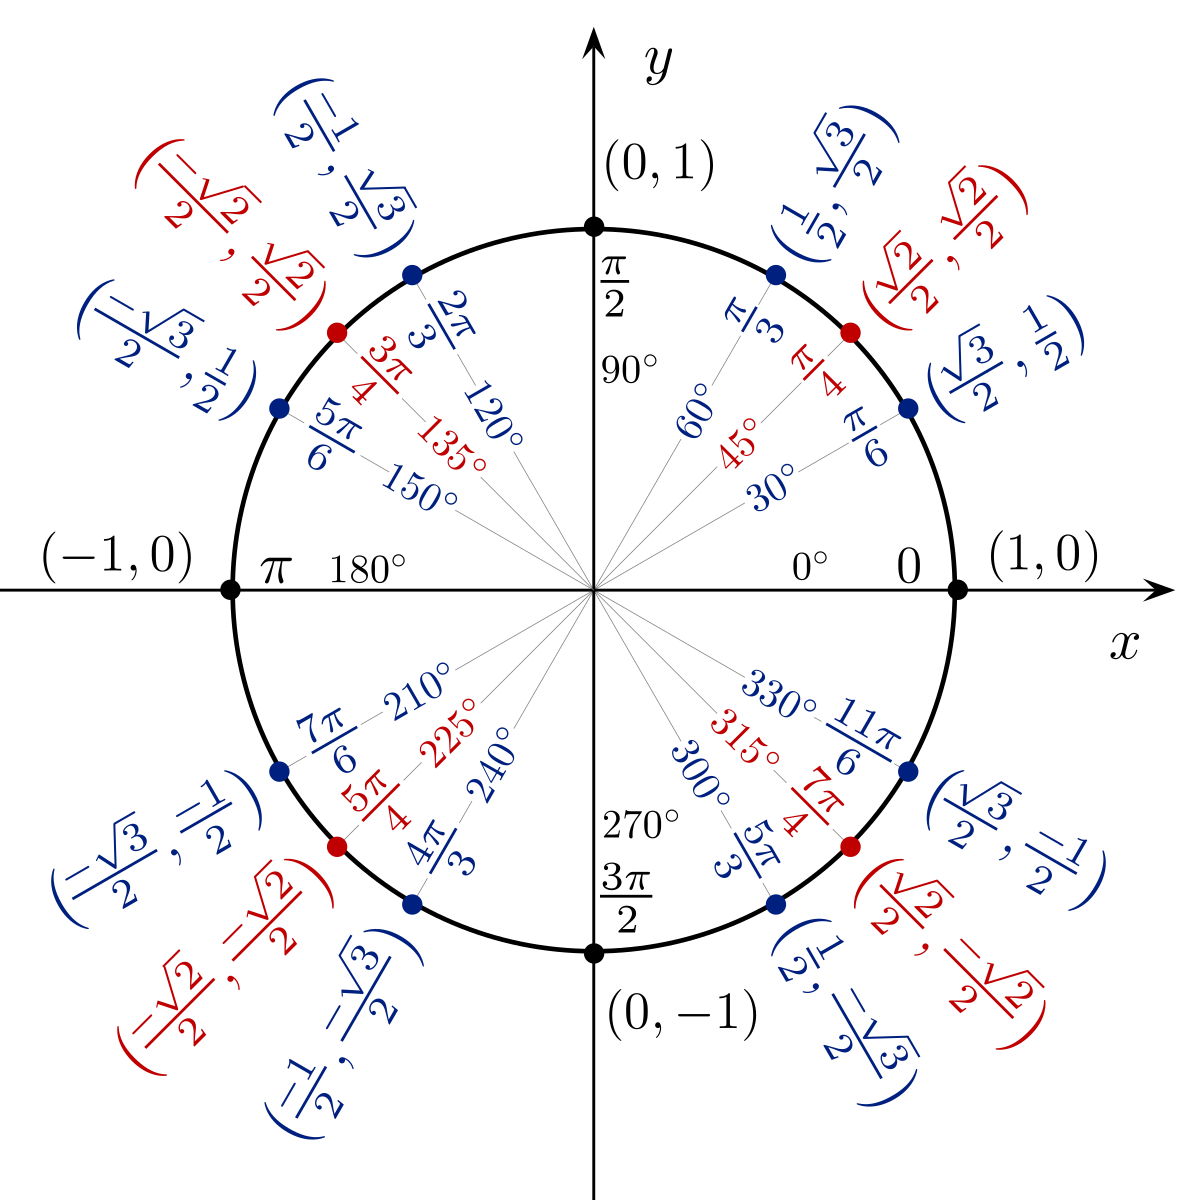
\includegraphics[width = 18em]{kreis}
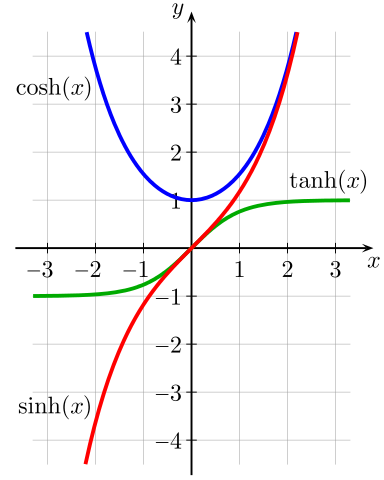
\includegraphics[width = 18em]{hyp}

\begin{Rechenregeln}{Rechenregeln Komplexe Zahlen}{}
    Imaginäre Einheit: \(i^{2} = -1\) \\
    Eulersche Formel: \( e^{i\varphi} = \cos(\varphi) + i\sin(\varphi) \), \(e^{i\varphi} = \cis(\varphi)\), \(\vert e^{i\varphi}\vert = 1\)	\\
    \begin{tabular}{|l|l|l|}
        \hline
        \(z\) & $ z = x + iy  \left\{
        \begin{array}{l}
        \text{x: Realteil}\\ \text{y: Imaginärteil}
        \end{array}
        \right. $  & \(z = r \cdot e^{i\varphi} = r \cdot \cis(\varphi)  \)\\ 
        \hline
        \(\overline{z}\) & \(\overline{z} = x - iy\) & \(z = r \cdot e^{-i\varphi}\)\\ 
        \hline
        \(\vert z \vert\) & \(\vert z \vert = \sqrt{z \cdot \overline{z}} = \sqrt{x^{2} + y^{2}}\) & \(\vert z \vert = r =\sqrt{z \cdot \overline{z}}\)\\ 
        \hline
        \(z_1 + z_2\) & \(x_1+x_2 + i(y_1+y_2)\) & \\
        \hline
        \(z_1 - z_2\) & \(x_1-x_2 + i(y_1-y_2)\) & \\
        \hline
        \(z_1 \cdot z_2\) & \((x_1x_2 - y_1y_2) + i(x_1y_2 + x_2y_1)\) & \(r_1 \cdot r_2 \cdot 
        e^{i(\varphi_1+\varphi_2)}\)\\
        \hline
        \(\frac{z_1}{z_2}, z_2 \neq 0\) & \(\frac{z_1 \cdot \overline{z_2}}{\vert z_2 \vert ^{2}} = \frac{(x_1x_2+y_1y_2)+i(x_2y_1-x_1y_2)}{x_2^{2}+y_2^{2}} \) & \(\frac{r_1}{r_2} \cdot e^{i(\varphi_1 - \varphi_2)}\)\\
        \hline
        \(\frac{1}{z}, z \neq 0\) & \(\frac{\overline{z}}{\vert z \vert ^{2}} = \frac{(x)+iy}{x^{2}+y^{2}} \) & \(\frac{1}{r} \cdot e^{-i\varphi}\)\\
        \hline
    \end{tabular}\\
    \begin{tabular}{|l|l|}
        \hline
        \(z^{n}\) & \(r^{n} \cdot (\cos(n\cdot \varphi)+ i \sin(n \cdot \varphi)) = r^{n} \cdot e^{in\varphi}\)\rule{0pt}{2.6ex}\\
        \hline
        \(\sqrt[n]{z}\) & \(\sqrt[n]{r}\cdot(\cos(\frac{\varphi + 2\pi k}{n})) + i\sin(\frac{\varphi + 2 \pi k }{n}), \ k = 0, 1, ..., n-1 \) \rule{0pt}{2.6ex}\\
        \hline
    \end{tabular}
    \begin{tabular}{|l|l|l|l|}
        \hline \(i^{0}\) & \(i^{1}\) & \(i^{2}\) & \(i^{3}\)\\
        \hline \(1\) & \(i\) & \(-1\) & \(-i\)\\
        \hline
    \end{tabular}
\end{Rechenregeln}

\begin{Rechenregeln}{Allgemeine Rechenregeln}{}
    \textbf{Betrag:} \\
    \(\vert ab \vert = \vert a \vert \vert b\vert \) \abstand 
    \(\vert \frac{a}{b} \vert = \frac{\vert a \vert}{ \vert b\vert} \) \abstand
    \(\vert a + b \vert \le \vert a \vert + \vert b \vert\) \\
    \\
    \textbf{Potenzen:} \\
    \(x = \sqrt[n]{a} 	\Leftrightarrow\ (x^{n}  = a \ \text{und } x \ \ge 0)\) \abstand
    \(\sqrt[n]{-a} = - \sqrt[n]{a}, \ a \ge 0\) \abstand
    \(a^{-n} = \frac{1}{a^{n}} = (\frac{1}{a})^{n}\) \abstand \(a^{\frac{1}{n}} = \sqrt[n]{a}\) \abstand \(\sqrt{ab} = \sqrt{a}\sqrt{b}\)\abstand \(a^{\frac{m}{n}} = \sqrt[n]{a^{m}}\) \abstand
    \( \sqrt{\frac{a}{b}} = \frac{\sqrt{a}}{\sqrt{b}} \) \abstand \( a^{x} = e^{x \cdot \ln a}\) \abstand 
    \(\sqrt[n]{a^{-m}} = \frac{1}{\sqrt[n]{a^{m}}}\)
    \(a^{m}a^{n} = a^{m+n} \) \abstand \(\sqrt[n]{a^{m}} = \sqrt[kn]{a^{km}}\) \abstand \(\frac{a^{m}}{a^{n}} = a^{m-n}\)
    \\ \( \sqrt[n]{\sqrt[k]{a}} = \sqrt[nk]{a}\) \abstand  \((a^{m})^{n} = a^{mn}\) \abstand \(\sqrt[n]{a}\sqrt[n]{b} = \sqrt[n]{ab}\) 
    \abstand \(a^{n}b^{n} = (ab)^{n}\) \abstand \(\frac{\sqrt[n]{a}}{\sqrt[n]{b}} = \sqrt[n]{\frac{a}{b}}\) 
    \abstand \(\frac{a^{n}}{b^{n}} = (\frac{a}{b})^{n}\) 
\end{Rechenregeln}

\begin{Rechenregeln}{Sinus und Cosinus}{}
    \begin{tabular}{|c@{\hspace{3pt}}|c@{\hspace{3pt}}|c|c|c|c|c|c|c|c|}
        \hline
        Grad &$0^\circ$ &$30^\circ$ &$45^\circ$ &$60^\circ$ &$90^\circ$ &$120^\circ$ &$135^\circ$ &$150^\circ$ &$180^\circ$\\
        \hline
        $\varphi$ &$0$ &$\frac{\pi}{6}$ &$\frac{\pi}{4}$ &$\frac{\pi}{3}$ &$\frac{\pi}{2}$ &$\frac{2\pi}{3}$ &$\frac{3\pi}{4}$ &$\frac{5\pi}{6}$ &$\pi$\\
        \hline
        $\sin(\varphi)$ &$0$ &$\frac{1}{2}$ &$\frac{\sqrt{2}}{2}$ &$\frac{\sqrt{3}}{2}$ &$1$ &$\frac{\sqrt{3}}{2}$ &$\frac{\sqrt{2}}{2}$ &$\frac{1}{2}$ &$0$\\
        \hline
        $\cos(\varphi)$ &$1$ &$\frac{\sqrt{3}}{2}$ &$\frac{\sqrt{2}}{2}$ &$\frac{1}{2}$ &$0$ &$-\frac{1}{2}$ &$-\frac{\sqrt{2}}{2}$ &$-\frac{\sqrt{3}}{2}$ &$-1$\\
        \hline
        $\tan(\varphi)$ &$0$ &$\frac{\sqrt{3}}{3}$ &$1$ &$\sqrt{3}$ &$\pm \infty$ &-$\sqrt{3}$ &$-1$ &$-\frac{\sqrt{3}}{3}$ &$0$\\
        \hline 
    \end{tabular}
    \begin{itemize}
    \item $\sin(x \pm y) = \sin(x)\cos(y) \pm \cos(x)\sin(y)$
    \item $\cos(x \pm y) = \cos(x)\cos(y) \mp \sin(x)\sin(y)$
    \item $\sin(x+y)\sin(x-y) = \cos^2(y) - \cos^2(x) = \sin^2(x) - \sin^2(y)$
    \item $\cos(x+y)\cos(x-y) = \cos^2(y) - \sin^2(x) = \cos^2(x) - \sin^2(y)$
    \item $\sin{x}\cos{y} = \frac{1}{2}(\sin(x+y) + \sin(x-y))$ 
    \item $\cos{x}\cos{y} = \frac{1}{2}(\cos(x+y) + \cos(x-y))$
    \item  $\sin{x}\sin{y} = \frac{1}{2}(\cos(x-y)-\cos(x+y))$
    \item $\cos(x)^2 + \sin(x)^2 = 1$
    \item $\cos(\pi-x) = -\cos(x)$, $\sin(\pi-x) = \sin(x)$
    \item $\cos(x+\pi) = -\cos(x)$, $\sin(x+\pi) = -\sin(x)$
    \item $\cos(2x) = \cos^2(x) - \sin^2(x) = 1-2\sin^2(x) = 2\cos^2(x) - 1$
    \item $\sin(2x) = 2\sin(x)\cos(x)$ \abstand $\tan(2x) = \frac{2\tan(x)}{1-\tan^2(x)}$
    \item $\sin(\frac{x}{2}) = \sqrt{\frac{1-\cos(x)}{2}}$ \abstand $\cos(\frac{x}{2}) = \sqrt{\frac{1+\cos(x)}{2}}$
    \item $\tan(\frac{x}{2}) = \frac{1-\cos(x)}{\sin(x)} = \frac{\sin(x)}{1+\cos(x)}$ \abstand $\cot(\frac{x}{2}) = \frac{1+\cos(x)}{\sin(x)} = \frac{\sin(x)}{1-\cos(x)}$
    \item $\sin^2(x) = \frac{1-\cos(2x)}{2}$
    \abstand $\cos^2(x) = \frac{1+\cos(2x)}{2}$
    \item $\sin^3(x) = \frac{3\sin(x) - \sin(3x)}{4}$ 
    \abstand $\cos^3(x) = \frac{3\cos(x) + \cos(3x)}{4}$
    \item $\tan(\pi + x) = \tan(x)$
    \item $-\sin(-x) = \sin(x), \cos(-x) = \cos(x), \tan(-x) = -\tan(x)$
    \item Für alle $(a,b)\in \R^2$, sodass $a^2+b^2 = 1$, gibt es $x\in\R$, sodass $a = \cos(x)$, $b = \sin(x)$.
    \item $\sin(x) = \frac{2\tan(x/2)}{1+\tan^2(x/2)}$
    \abstand $\cos(x) = \frac{1-\tan^2(x/2)}{1+\tan^2(x/2)}$
    \item $\sin(x) = \frac{e^{ix} - e^{-ix}}{2i}$
    \abstand $\cos(x) = \frac{e^{ix} + e^{-ix}}{2}$
    \item $\int_0^{2\pi} \sin(t)\cdot \cos(t) dt = \int_0^{2\pi} \sin(t) dt = \int_0^{2\pi} \cos(t) dt = 0$
    \item $\int \sin^2(x) dx = \frac{1}{2} (x-\sin(x) \, \cos(x))$
    \item $\int \cos^2(x) dx = \frac{1}{2} (x+\sin(x) \, \cos(x))$
    \item $\int x \sin(x) dx = \sin (x)-x \cos (x)$
    \item $\int x \cos(x) dx = x \sin (x)+\cos (x)$
    \item \(\sin(\arccos(x)) = \sqrt{1-x^{2}}\) \abstand \(\sin(\arctan(x)) = \frac{x}{\sqrt{1+x^{2}}}\) 
    \item \(\cos(\arctan(x)) = \frac{1}{\sqrt{1+x^{2}}}\) \abstand \(\cos(\arcsin(x)) = \sqrt{1-x^{2}}\) 
    \item \(\tan(\arcsin(x)) = \frac{x}{\sqrt{1-x^{2}}}\) \abstand \(\tan(\arccos(x)) = \frac{\sqrt{1-x^{2}}}{x}\)
    \item $\cosh(x) := \frac{e^x + e^{-x}}{2}$ \abstand $\sinh x := \frac{e^x - e^{-x}}{2}$ \abstand $\tanh x := \frac{e^x - e^{-x}}{e^x + e^{-x}}$
    \item $\sinh(z) = -\sinh(-z)$ \abstand $\cosh(z) = \cosh(-z)$ 
    \item $\sinh(z) = \sinh(z + 2\pi i)$ \abstand $\cosh(z) = \cosh(z+ 2\pi i)$
    \item $\sinh(z_1 \pm z_2) = \sinh(z_1) \cdot \cosh(z_2) \pm \sinh(z_2) \cdot \cosh(z_1)$
    \item $\sinh(z_1 \pm z_2) = \cosh(z_1) \cdot \cosh(z_2) \pm \sinh(z_2) \cdot \sinh(z_1)$
    \item $\tanh(z_1 \pm z_2) = \frac{\tanh(z_1) \pm \tanh(z_2)}{1 \pm \tanh(z_1)\cdot \tanh(z_2)}$
    \end{itemize}
\end{Rechenregeln}

\begin{Rechenregeln}{Ableitung}{}
    \begin{itemize}
        \item \textbf{Summenregel} $(f(x)+g(x))' = f'(x) + g'(x)$
        \item \textbf{Faktorregel} $(c\cdot f(x))' = c\cdot f'(x)$
        \item \textbf{Produktregel} $(f(x)\cdot g(x))' = f'(x)g(x) + f(x)g'(x)$
        \item \textbf{Quotientenregel} $\left(\frac{f(x)}{g(x)}\right)' = \frac{f'(x)g(x) - f(x)g'(x)}{g^2(x)}(g\neq 0)$
        \item \textbf{Kettenregel} $(f(g(x)))' = (f\circ g)' = f'(g(x))g'(x)$
    \end{itemize}
\end{Rechenregeln}

\begin{Rechenregeln}{Integration}{}
    \begin{itemize}
    \item \textbf{Summe/Differenz:} $\int_a^b (f(x) +/- g(x)) xd = \int_a^b f(x) +/- \int_a^b g(x)$
    \item \textbf{Konstanter Faktor:} $\int_a^b c\cdot f(x)dx = c\cdot \int_a^b f(x)dx$
    \item \textbf{Partielle Integration:} $\int_a^b f'(x)\cdot g(x)dx = \left[f(x)g(x)\right]_a^b - \int_a^b f(x)g'(x)$
    \item \textbf{Substitution:} $\int_{\phi(a)}^{\phi(b)} f(x)dx = \int_a^b f(\phi(t))\phi '(t) dt$
    \item \textbf{$a+c, b+c \in I$} $\int_a^b f(t+c)dt = \int_{a+c}^{b+c} f(x)dx$
    \item \textbf{$ca,cb\in I$: } $\int_a^b f(ct)dt = \frac{1}{c}\int_{ca}^{cb} f(x)dx$
    \item \textbf{Logarithmus: }\;(f stetig diffbar) $\int\frac{f'(t)}{f(t)}dt = \log(|f(x)|)$, bzw. $\int_a^b\frac{f'(t)}{f(t)}dt = \log(f(|b|)) - \log(f(|a|))$
    \item \textbf{Partialbruch: }\\
     $\frac{2x^6-4x^5+5x^4-3x^3+x^2+3x}{(x-1)^3(x^2+1)^2} = \frac{A}{x-1}+\frac{B}{(x-1)^2}+\frac{C}{(x-1)^3}+\frac{Dx+E}{x^2+1}+\frac{Fx+G}{(x^2+1)^2}$
    \end{itemize}
\end{Rechenregeln}

\begin{Rechenregeln}{Limes}{}
    \begin{itemize}
    \item $\lim_{x\to 0} \arctan(x) = 0$, $\lim_{x\to\infty} \arctan(x) = \frac{\pi}{2}$
    \item $\lim_{x\to 0} \tan(x) = 0$, $\lim_{x\to\infty} \tan(x) = \infty$, $\lim_{x\to\frac{\pi}{2}} \tan(x) = \infty$
    \item $\Lim{n \rightarrow \infty}{(1+\frac{x}{n})^{n}} = e^{x}$ \abstand $\Lim{n \rightarrow \infty}{(1+\frac{1}{n})^{n}} = \LimNI{(1+n)^{\frac{1}{n}}} = e$ 
    \item $\LimXO{\frac{a^{x}-1}{x}} = \ln(a)$ \abstand \(\LimXO\frac{\log_a(1+x)}{x} = \frac{1}{\ln(a)}\) \abstand \(\LimXO{\frac{1-\cos(x)}{x}} = 0\) 
    \item \( \LimXO{\frac{1-\cos(x)}{x^{2}}} = \frac{1}{2} \) \abstand \( \LimXO{\frac{\tan(x)}{x}} = 1\) \abstand \( \LimXO{\frac{\sin(x)}{x}} = 1 = \frac{x}{\sin(x)}\) 
    \item \(\LimNI{\frac{n!}{n^{n}}} = 0\) \abstand \(\LimNO{\frac{e^{n} -1}{n}} = 1\) \abstand \(\LimNI{\sqrt[n]{n!}} = \infty\) \abstand \(\LimNI {\sqrt[n]{n}} = 1\)
    \end{itemize}
    \textbf{Entscheidbare Situationen}
    $\frac{1}{0} = \infty$ \abstand $\frac{1}{\infty} = 0$ \abstand $\infty + \infty = \infty$ 
    \abstand $0 + \infty = \infty$ \abstand $0^{\infty} = 0$ \abstand $\infty^{\infty} = \infty$
\end{Rechenregeln}

\begin{Rechenregeln}{Reihen}{}
    \begin{itemize}
        \item $\sum_{k=0}^{\infty} aq^{k} = a + aq + aq^{2} +... = \frac{a}{1-q}$ (geometrische Reihe)
        \item $\sum_{k=0}^{\infty} (k+1)q^{k} = 1 + 2q + 3q^{2} +... = \frac{1}{(1-q)^{2}}, \ \vert q \vert < 1$ 
        \item $\sum_{k=0}^{\infty} \frac{(-1)^{k}}{2k+1} = 1 - \frac{1}{3} + \frac{1}{5} - \frac{1}{7} + ... = \frac{\pi}{4}$
        \item $\sum_{k=1}^{\infty} \frac{1}{k^{2}} = 1 + \frac{1}{2^{2}} + \frac{1}{3^{2}} + \frac{1}{4^{2}} + ... = \frac{\pi^{2}}{6}$
        \item $\zeta(a) = \sum_{k=0}^{\infty} \frac{1}{k^{a}} \text{ist konvergent} \iff a>1$
        \item $\sum_{k=0}^{\infty} \frac{1}{k!} = 1+\frac{1}{1!} + \frac{1}{2!} + \frac{1}{3!} + ... = e$
        \item $\sum_{k=0}^{\infty} \frac{(-1)^{k}}{k!} = 1 - \frac{1}{1!} + \frac{1}{2!} - \frac{1}{3!} + ... = \frac{1}{e}$
        \item $\frac{1}{1 \pm x} = 1 \mp x + x^2 \mp x^3 + x^4 \mp ...$
        \item $\frac{1}{(1 \pm x)^2} = 1 \mp 2x + 3x^2 \mp 4x^3 + 5x^4 \mp ...$
        \item $\sqrt{1 \pm x} = 1 \pm \frac{x}{2} - \frac{\scriptstyle{1\cdot 1}}{\scriptstyle{2 \cdot 4}}x^2 \pm \frac{\scriptstyle{1\cdot 1 \cdot 3}}{\scriptstyle{2 \cdot 4 \cdot 6}}x^3 - \frac{\scriptstyle{1 \cdot 1 \cdot 3 \cdot 5}}{\scriptstyle{2 \cdot 4 \cdot 6 \cdot 8}}x^4 \pm \scriptstyle\cdots$
        \item $\exp(x) = \sum_{n=0}^{\infty} \frac{x^{n}}{n!} = 1 + x + \frac{x^{2}}{2!} + \frac{x^{3}}{3!} + ....$
        \item $\sin(x) =  \sum_{n=0}^{\infty} (-1)^{n}\frac{x^{2n+1}}{(2n +1)!} = x - \frac{x^{3}}{3!} + \frac{x^{5}}{5!} - \frac{x^{7}}{7!} + ...$ 
        \item $\cos(x) =  \sum_{n=0}^{\infty} (-1)^{n}\frac{x^{2n}}{(2n)!} = 1 - \frac{x^{2}}{2!} + \frac{x^{4}}{4!} - \frac{x^{6}}{6!} + ...$ 
        \item $\sinh(x) = \sum_{n=0}^{\infty} \frac{x^{2n+1}}{(2n+1)!} = x + \frac{x^3}{3!} + \frac{x^5}{5!} + ...$
        \item $\cosh(x) = \sum_{n=0}^{\infty} \frac{x^{2n}}{(2n)!} = 1 + \frac{x^2}{2!} + \frac{x^4}{4!} + ...$
        \item $\tan(x) = 1 + \frac{x^3}{3} + \frac{2x^5}{15} + ...$
        \item $\tanh(z) = 1 \pmb{-} \frac{z^3}{3} \pmb{+} \frac{2z^5}{15} \pmb{-} ...$
        \item $\ln(1+z) = \sum_{k=1}^{\infty} \frac{(-1)^{k+1}}{k}z^k = z - \frac{z^2}{2} + \frac{z^3}{3} + ...$
        \item $(1+z)^\alpha = \sum_{k=0}^{\infty}  \binom{\alpha}{k} z^k = 1 + \alpha z + \frac{\alpha(\alpha - 1)}{2!} z ^ 2 + ...$
    \end{itemize}
\end{Rechenregeln}

\begin{Diverses}{}{}
    \begin{itemize}
    \item Kreisgleichung $(x - x_0)^2 + (y - y_0)^2 = r^2$
    \item Ellipsengleichung $\frac{(x-x_0)^2}{a^2} + \frac{(y-y_0)^2}{b^2} = 1$
    \item Mitternachtsformel $x_{1, 2} = \frac{-b \pm \sqrt{b^2 - 4ac}}{2a}$
    \item Matrix Determinante $\begin{vmatrix}
        a & b\\
        c & d
    \end{vmatrix} = ad-bc$
    \item Matrix Invertierbarkeit: Eine quadratische Matrix ist genau dann invertierbar, falls die Determinante $\neq 0$.
    \item Skalarprodukt $x \cdot y = \sum_{i=1}^n x_i y_i$
    \item Kreuzprodukt $a \times b = (a_2b_3-a_3b_2, ~~~ a_3b_1-a_1b_3, ~~~ a_1b_2-a_2b_1)^\top$
    \end{itemize}
\end{Diverses}

\begin{Rechenregeln}{Stammfunktionen, Ableitungen}{}
    \begin{center}
        $\textbf{differenzierbar }\implies\textbf{ stetig }\implies \textbf{ integrierbar}$\\
    \end{center}
    \begin{longtable}{l|l|l}
        $\mathbf{f'(x)}$ & $\mathbf{f(x)}$ & $\mathbf{F(x)}$ \\[0.5em] \hline
        0 & c ($c\in\R)$ & $cx$ \\[0.5em]
        $c$ & $cx$ &$\frac{c}{2}x^2$ \\[0.5em]
        $r\cdot x^{r-1}$ & $x^r (r\in \R \backslash \{-1\}$ & $\frac{x^{r+1}}{r+1}$ \\[0.5em]
        $\frac{-1}{x^2} = -x^{-2}$ & $\frac{1}{x}=x^{-1}$ & $\log |x| $ \\[0.5em]
        $\frac{1}{2 \sqrt{x}} = -x^{-2}$ & $\sqrt{x} = x^{\frac{1}{2}}$ & $\frac{2}{3}x^{\frac{3}{2}}$ \\[0.5em]
        $\cos x$ & $\sin x$  & $-\cos x$ \\[0.5em]
        $-\sin x$ & $\cos x$ & $\sin x$\\[0.5em]
        $1+\tan^2x = \frac{1}{\cos^2x}$ & $\tan x$ & $-\log|\cos x|$\\[0.5em]
        $-\frac{1}{\sin^2(x)}$ & $\cot x$ & $\log|\sin x|$\\[0.5em]
        $e^x$ & $e^x$ & $e^x$\\[0.5em]
        $c\cdot e^{cx}$ & $e^{cx}$ & $\frac{1}{c}e^{cx}$\\[0.5em]
        $\log a \cdot a^x$ & $a^x$ & $\frac{a^x}{\log a}$\\[0.5em]
        $\frac{1}{x}$ & $\log|x|$ & $x(\log|x|-1)$ \\[0.5em]
        $\frac{1}{\log a\cdot x}$ & $\log_a |x|$ & $\frac{x}{\log a}(\log|x|-1)$\\[0.5em]
         & & = $x(\log_a|x|-\log_ae)$\\[0.5em]
        $\frac{1}{\sqrt{1-x^2}}$ & $\arcsin x$ & $x\arcsin x + \sqrt{1-x^2}$\\[0.5em]
        $-\frac{1}{\sqrt{1-x^2}}$ & $\arccos x$ &  $x\arccos x - \sqrt{1-x^2}$\\[0.5em]
        $\frac{1}{1+x^2}$ & $\arctan x$ & $x\arctan x - \frac{1}{2}\log(1+x^2)$\\[0.5em]
        $\sinh(x)$ & $\cosh(x)$ & - \\[0.5em]
        $\cosh(x)$ & $\sinh(x)$ & -\\[0.5em]
        $\frac{1}{\cosh^2(x)}$ & $\tanh(x)$ & $\log(\cosh(x))$\\[1em]
        $2 \sin(x)\cos(x)$ & $\sin^2(x)$ & $\frac{1}{2}(x-\sin(x)\cos(x))$ \\[.5em]
        $-2\sin(x)\cos(x)$ & $\cos^2(x)$ & $\frac{1}{2}(x+\sin(x)\cos(x))$ \\[.5em]
        $\frac{2 \sin(x)}{\cos^3(x)}$ & $\tan^2(x)$ & $\tan(x) - x$\\[.5em]
        \(\frac{1}{\sqrt {x^2+1}}\)& \(\operatorname{arsinh} x\) & \(x \operatorname{arsinh} x -\sqrt{x^2+1}\)\\
        \(\frac{1}{\sqrt {x^2-1}} \quad (x>1)\)&\(\operatorname{arcosh} x\) & \(x \operatorname{arcosh} x -\sqrt{x^2-1}\)\\
        \(\frac{1}{1-x^2} \quad (\left| x \right|<1)\)&\(\operatorname{artanh} x\) & \(x \operatorname{artanh} x +\frac{1}{2}\ln{\left(1-x^2\right)}\)\\
        \(\frac{1}{1-x^2} \quad (\left| x \right|>1)\)&\(\operatorname{arcoth} x\) & \(x \operatorname{arcoth} x +\frac{1}{2}\ln{\left(x^2-1\right)}\)\\ 
    \end{longtable}
\end{Rechenregeln}

